\section{İLETİM ORTAMLARI}
Temelde atmosfer ve kablo olmak üzere iki farklı iletim ortamı mevcuttur. Atmosferde RF (radyo frekans) dalgalarını kullanarak  iletişim gerçekleşir.
Kablolarda ise genellikle fiberoptik ve bakır kablo kullanılmaktadır.

\subsection{İKİ TELLİ BAKIR TELEFON HATTI }
Telefon iletişimini sağlamak için tasarlanmıştır. Temel bant ve geniş bant internet hizmeti verilmektedir.
Analog modülasyon teknikleriyle en fazla 56 k b/s'lik band genişliği sağlar. xDSL teknolojileriyle 25 Mb/s'lik bant genişliğine ulaşmaktadır.
\begin{figure}[ht]
    \centering
    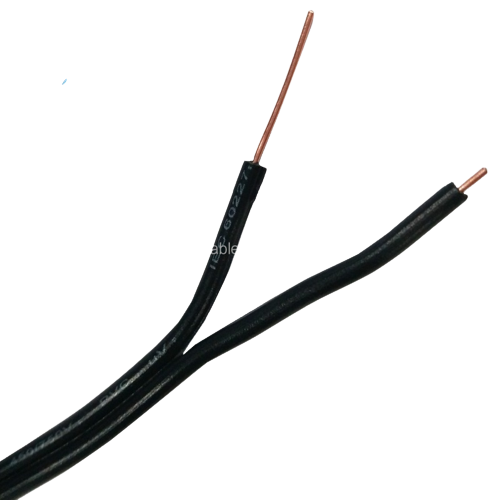
\includegraphics[width=8cm,height=6cm]{images/ikitellibakirkablo}
    \caption{İki telli Bakir Kablo}
    \label{fig:iki_telli_bakir_kablo}
\end{figure}

\subsection{KOAKSİYEL (COAXIAL) KABLO}
Genellikle elektriksel gürültünün yoğun olduğu şartlarda kullanılırdı.Yalıtkan bir tüpün içerisinde giden bir tel ve tüpün dışına sarılmış kafes şeklinde teller vardır.
Yerel ağlarda (LAN) 180m'de(max) 10M b/s bant genişliği sağlar. Bu kullanımı 10 Base 2 olarak bilinir. Daha sonra 500 m mesafede çalıştırılacak hale getirilir. 10 Base 2 ismiyle standartlaştırılmıştır. 50 ohm'luk direnç değeri vardır.
BNC tarzında konnektörler kullanılır. Günümüzde LAN'da hiç kullanılmamaktadır. Sebebi hem 10 Mb/s hızının çok düşük olması, hem de UTP kablolar kadar ekonomik ve işlevsel olmamasıdır.
Bilgisayar ağlarında doğrusal (bus) topolojilerde kullanılmıştır.

\begin{figure}[H]
    \centering
    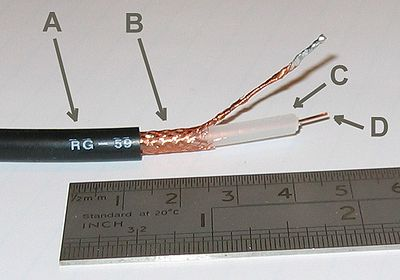
\includegraphics[width=8cm]{images/400px-RG-59}
    \caption{Koaksiyel Kablo}
    \label{fig:kooksiyel_kablo}
\end{figure}


\section*{AĞ TOPOLOJİLERİ }
\begin{figure}[H]
    \centering
    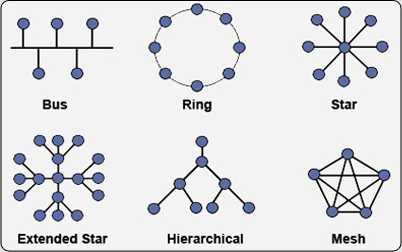
\includegraphics[width=8cm]{images/62_ağ_topolojisi}
    \caption{Topolojiler}
    \label{fig:topolojiler}
\end{figure}
 % bu kısım notlarda yok topoloji nedir kısmını ben ekledim.
Ağ topolojileri nedir sorusunun en net cevabı, "bir ağı oluşturan cihazların fiziksel ve mantıksal yerleşimidir". Network Topology (Ağ Topolojisi) Yerel Ağ Alanı (LAN) içerisinde bulunan bilgisayarların fiziksel ve mantıksal yerleşimini ifade eder. Fiziksel Topoloji ağ içerisinde bulunan tüm cihazların birbirlerine nasıl bağlanacağını ve bağlantı için ne tür kablo kullanacağını belirtirken Mantıksal Topoloji bu cihazların nasıl haberleşeceğini belirtir ve bu cihazları ortak bir protokol altında birleştirir. Kullanılmak istenen Ağ Teknolojisine göre farklı ağ topolojileri kullanılmaktadır.
Fiziksel Topolojinin 6 farklı çeşidi vardır. Bunlar Bus(Yol), Ring(Halka), Yıldız(Star), Ext Star(Gelişmiş Yıldız), Mesh(Örgü) ve Tree(Ağaç) topolojileridir. Broadcast(Yayın) ve Token Passing(İz) mantıksal topolojilere birer örnektir.

\subsection*{DOĞRUSAL (BUS) TOPOLOJİ}
Doğrusal bir hat üzerinde bilgisayarların T konnektörlerle bağlanması şeklinde kurulur. Hattın her iki ucunda sonlandırıcı kullanmak zorunludur. Koaksiyel kablo kullanılır. Ağın herhangi  bir noktasında arıza olması durumunda ağın tamamı çöker.Ağdaki veri trafiği tüm uçlara gider. Herkes herkesin trafiğini görebilir. Bu yüzden çok fazla \textbf{çakışma (colision)} olur.
\begin{figure}[H]
    \centering
    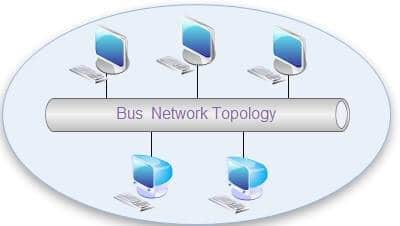
\includegraphics[width=8cm]{images/bus-topolojisi}
    \caption{Bus Topolojisi}
    \label{fig:bustopolojisi}
\end{figure}
\subsection*{HALKA (RING) TOPOLOJİ}
Doğrusal topolojiye benzer. Sonlandırıcı kullanılmaz. Hattın iki ucu birleşiktir. Hatta sanal  bir jeton dolaşır(token).Jeton sırası gelen bilgisayar, jeton boş ise göndereceği veriyi hatta yerleştirir.
Bilgisayarlar sırayla veri gönderdiklerinden çakışma daha azdır.Günümüzde hiç kullanılmamaktadır. Herkes herkesin verisini kullanabilmektedir.
%bu fotoğraf en alta geçiyor düzeltilecek
\begin{figure}[H]
    \centering
    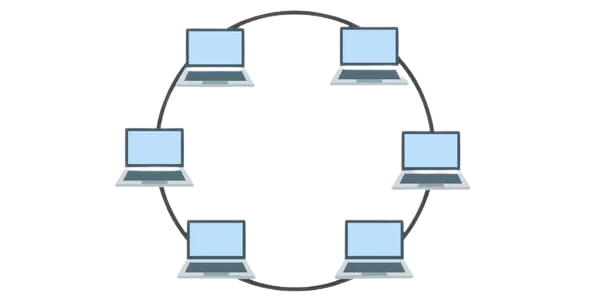
\includegraphics[width=8cm]{images/ring-topology-removebg-preview}
    \caption{Halka-Ring Topolojisi}
    \label{fig:halka_topolojisi}
\end{figure}

\subsection*{YILDIZ (STAR) TOPOLOJİ}
Merkezde dağıtıcı bir cihaz olur.
Buradan tüm bilgisayarlara birer kablo gider.
Ağın bir noktasındaki arıza sadece ilgili bilgisayarın ağ bağlantısına zarar verir.
Genellikle \textbf(bükümlü çift (twisted pair,xtp)) kullanılır.
Trafiğin herkese mi gönderileceği ya da sadece ilgili uca mı gideceği dağıtıcıya bağlıdır.
Dağıtıcının performansı ve kabiliyeti ağı doğrudan etkiler.
Günümüzde en yaygın topolojidir.

\begin{figure}[H]
    \centering
    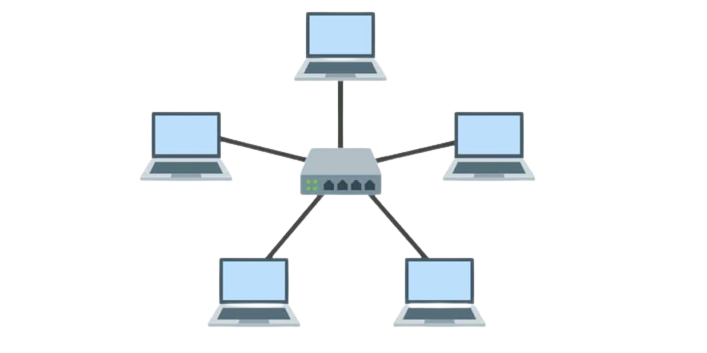
\includegraphics[width=8cm]{images/star-Topology-1024x512-removebg-preview}
    \caption{Yildiz-StarTopolojisi}
    \label{fig:yildiz_topolojisi}
\end{figure}

\subsection*{ÖRGÜ (MESH)TOPOLOJİ}

\begin{figure}[H]
    \centering
    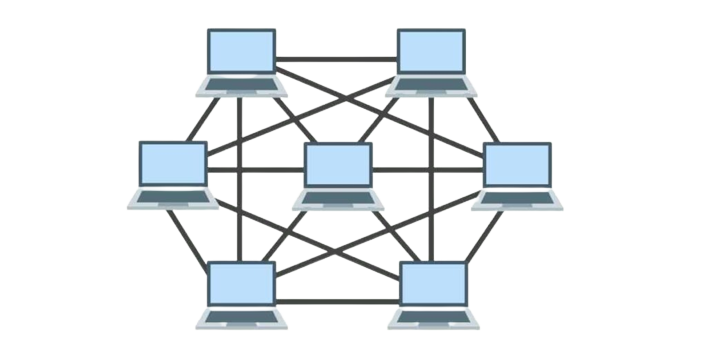
\includegraphics[width=12cm]{images/mesh-topology-1-1024x512-removebg-preview}
    \caption{Örgü-Mesh Topolojisi}
    \label{fig:Orgu_mesh_topolojisi}
\end{figure}
Uçları arasında birden fazla rota üzerinde haberleşme imkanı olan yapılardır.
Günümüzde genellikle farklı yıldız ağlar arasında yedekleme amacı olarak kullanılır.

\subsection{BÜKÜMLÜ ÇİFT KABLO}
İçerisinde 4 çift bakır kablo bulunur.Kabloların birbirleri üzerindeki direnç elektromanyetik etkisini azaltmak için ikişerli olarak sarılı durumundadırlar.
Örneğin: UTP,CAT5,Ethernet Kablosu
\begin{figure}[H]
    \centering
    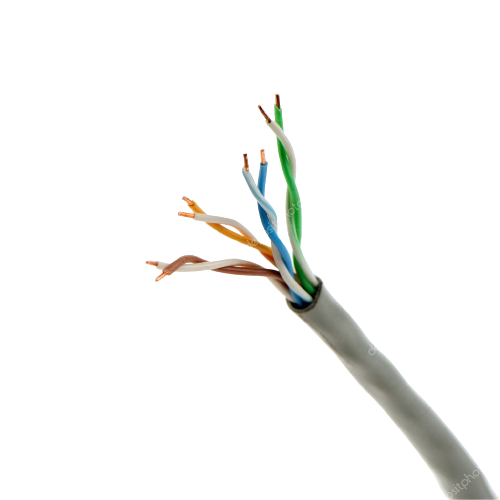
\includegraphics[width=6cm]{images/bukumlukablo}
    \caption{Bükümlü çift kablodan bir kesit}
    \label{fig:Bukumlu_cift_kablo}
\end{figure}

\subsubsection{UTP (UNSHILDED TWISTED PAIR) Korumasız Bükümlü Çift}
8 iletkenin her biri ince bir yalıtkan ile kaplanmıştır. En dışında tamamını kaplayan bir yalıtkan vardır.

\subsubsection{STP(SHİLDED TWİSTED PAİR)}
Her çiftin altında koruma (topraklama ) vardır.

\subsubsection{FTP(FOİLED TWİSTED PAİR )}
4 çiftin tamamının etrafında folyo koruma vardır.
\subsubsection {S/FTP }
İkisinin de özelliğini taşımaktadır.
    
\subsection{FREKANSLARINA GÖRE BÜKÜMLÜ ÇİFT KABLO}
\textbf{CAT:}\\
\textbf{CAT1-CAT3} \\
Telefon hatlarında bulunur.\\
\textbf{CAT5} \\
En yaygın kullanılan ağ kablosudur. Azami 100m mesafe ve 10Mb/s destekler.\\
\textbf{CAT6} \\
100 m mesafede 1G b/s destekler.\\
\textit{10 BASE T} Ethernet(Eth)\\
\textit{100 BASE T} Fast Ethernet(Fa,Fe)\\
\textit{1000 BASE T} Gigabit Ethernet(G,GE)\\
Bükümlü çift CAT5 VE CAT6 Kabloları  sonlandırmak için RJ-45 adı verilen konnektörler kullanılır.
Bu kablolar iki farklı iki şekilde sonlandırılabilir.\textbf{568-A,568-B}\\
Kablonun iki ucunun aynı standartlarla sonlandırılmasına \textbf{düz (Straight kablo)} denir. İki ucunda iki farklı standartta sonlandırılma yapılırsa \textbf{çapraz(cross-over)kablo } adı verilir.
\subsection{ÇAPRAZ VE DÜZ KABLO}
Düz kablo, bir bilgisayarı yönlendirici gibi bir ağ hub'ına bağlamak için yerel alan ağlarında kullanılan bir tür bükümlü çift kablodur. Bu tür kablolara bazen yama kablosu da denir ve bir veya daha fazla bilgisayarın kablosuz bir sinyal yoluyla bir yönlendiriciye eriştiği kablosuz bağlantılara bir alternatiftir. Aynı türden iki cihazı bağlamak için genellikle bir çapraz kablo kullanılır. Düz kablo ve çapraz kablo tasarımları aynı standartların ve kuralların çoğunu kullanır.

\begin{figure}[ht]
    \centering
    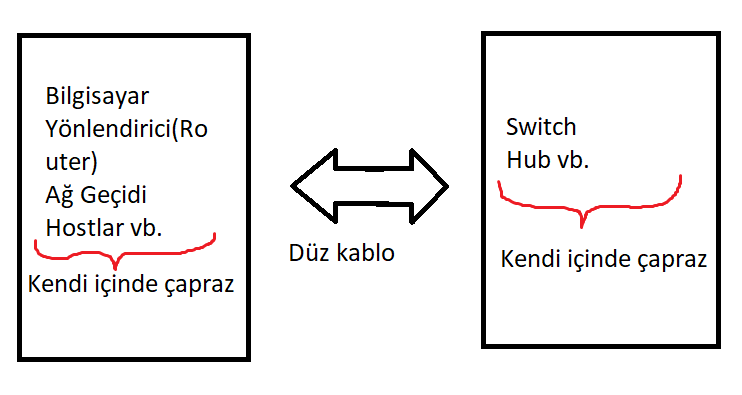
\includegraphics[width=8cm]{images/caprazduzz}
    \caption{kablolar}
    \label{fig:caprazduz_kablo}
\end{figure}

Yeni ağ cihazlarının tamamı MDI/MDIX adı verilen teknoloji sayesinde karşıdaki cihazın ne tarz bir cihaz olduğunu anlar ve hangi iletkenin ne amaçla kullanılacağını buna göre  düzenler. Diğerleri enerji göndermek için kullanılır.

\begin{figure}[ht]
    \centering
    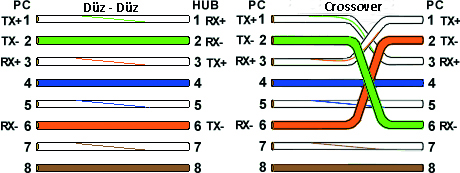
\includegraphics[width=10cm]{images/ethcable}
    \caption{kablolar-örnek}
    \label{fig:caprazduz_kablo_ornek_gosterim}
\end{figure}

\section*{FİBER OPTİK KABLOLAR}
Fiber optik kablolar, veri göndermek için ışık sinyallerini kullanmaktadır. Bu kablolar elektrik kablolarına benzer. Ancak elektrik kablolarından farklı olarak ışığı taşımak için kullanılan minimum bir adet fiber optik içeren bir kablo çeşididir.\\
Fiber optik kablolar çeşitli özelliklere ve avantajlara sahiptirler. Fiber optik kablonun farklı alanlarda  bu kadar sık tercih edilmesinin nedenleri kabloların bulundurduğu özellikler ve sunduğu bu avantajlardır. \\
\textbf{Fiber Optik Avantajları}\\
Elektrik parazitlerinden etkilenmez.\\
Sıcaklık değişimleri ve neme karşı dayanıklıdır.\\
Metalik kablolardan daha hafif ve daha küçüktürler.\\
Sinyal kaybı yok denecek kadar azdır ve sinyal güçlendirici ihtiyacını azaltır.\\
Sıcaklık değişimleri, su baskınları, şiddetli hava ve nem gibi çevresel parametrelere karşı dayanıklıdır.\\
Bu kablolarda iletim için ışığın yansımasını kullanılır. Böylelikle bu kablolar çok daha uzun mesafelere veri iletimi yapılabilirler.
Elektromanyetik enerji sızması meydana gelmediği için bilgi güvenliği sağlanmış olur.\\
Bu kablolar ile bilginin ekonomik, verimli ve hızlı bir şekilde ulaştırılması sağlanır.\\
\textbf{Fiber Optik Dezavantajları}\\
Sınırlı Uygulama — Fiber optik kablo sadece zeminde kullanılabilir ve zemini terk edemez veya mobil iletişim ile çalışamaz.\\
Düşük Güç — Işık yayan kaynaklar, düşük güçle sınırlıdır. Güç kaynağını iyileştirmek için yüksek güç yayıcıları bulunmasına rağmen, ek maliyet ekleyecektir.\\
Kırılganlık - Fiber optik, bakır tellere kıyasla daha kırılgandır ve hasara karşı daha hassastır. Fiber optik kabloları bükmemeli veya bükmemelisiniz.\\
Mesafe — Verici ve alıcı arasındaki mesafe kısa olmalı veya sinyali arttırmak için tekrarlayıcılara ihtiyaç duyulmalıdır.\\

\begin{figure}[H]
    \centering
    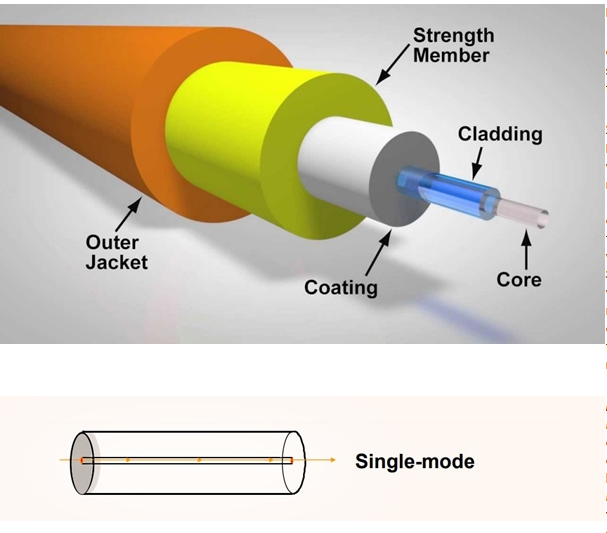
\includegraphics[width=8cm]{images/fiberoptik}
    \caption{fiberkablo}
    \label{fig:fiberoptikkablo}
\end{figure}

 Veri optik dalgalar arıcılığı ile ışığın yansıma kurallarına göre elde edilir.
 Elektiriksel sinyallerine göre mesafeye bağı zayıflama sinyalleri çok azdır.
 Bakır kablolarda olduğu gibi gerilim farkından kaynaklanan topraklama ihtiyacı yoktur.
 Fiberoptik kabloların yerel ağa bağlanmasında elektiriksel sinyal ile optik dalgalar arasında çevrilmesi gerekir.Verici tarafından ışık kaynağı olarak lazer diyod(led),alıcı tarafında ise fotodiyod ya da foto transistör kullanılır.
\subsection{FİBER OPTİK KABLO TÜRLERİ}
Single mod(SM) ve Mlti mod(MM) olmak üzere ikiye ayrılır\\
\textbf{Multi-Mode}\\
Bina ya da kampüs içi kısa mesafelerde tercih edilir.Optik dalga üretmek için Led kullanılır.Verici ve alıcı maliyetleri single moduna göre yarı yarıya azdır.
\textbf{Single-Mode}
Hem daha uzun mesafelerde hem de daha yüksek band genişliğine imkan sağlar.
Optik dalga üretmek için LazerDiyod kullanılır.Bu nedenle verici ve alıcı donanım maliyetleri daha fazladır.

\begin{figure}[ht]
    \centering
    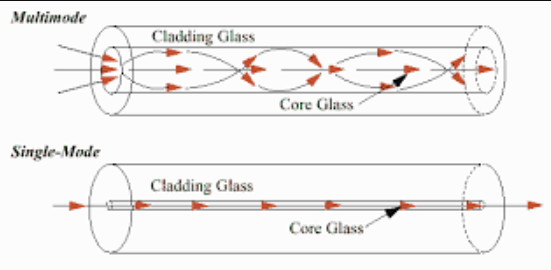
\includegraphics[width=10cm]{images/single-multimode}
    \caption{single-multimode}
    \label{fig:single_multi_mode}
\end{figure}
\subsection*{FİBER OPTİK ÇEVİRİCİLER}
*F/O CONVERTOR \\
*F/O TRANSREİVER (ALICI/VERİCİ)\\
*GBIC  (Switch modülü halindedir) \\
*STP  (Switch modülü halindedir) \\

\subsection*{YEREL AĞLAR (LAN)}
Kablo çekebileceğimiz (bize ait  olan ) yerler yerel ağlardır.
Ağlarda band genişliği ,protokol,topoloji gibi altarnetifler isteğe göre özelleştirilebilir.
Günümüz yerel ağlarında ethernet harici protokol kullanılmamamktadır.
\subsection*{ETHERNET PROTOKOLÜ}
İlk kez "INTEL VE XEROX" tarafından geliştirilmiştir.Daha sonra IEEE(Institue of Electrical and Electronical Enginner) tarafından 809.3 ismi ile standartlaştırılmıştır.
\subsection*{10 M b/s Ethernet Portları}
\textbf{10 Base 2 :} 10 sayısı 10 m b/s'yi ifade eder.Base sözcüğü temel bandı ifade eder.En sondaki kablo türüdür.2 olduğunda ince (thin) kooksiyel kablodur.\\
\textbf{10 Base 5 :} Sondaki 5 Kalın(thick) kooksiyel kablo olduğunu belirtir.\\
\textbf{10  Base T :}Bükümlü çift kablo olduğunu ifade eder.\\
\subsection*{100 M b/s ETHERNET PORTLARI}
\textbf{100 Base Tx :}Fast Ethernet Cat-5 kablo kullanılır.\\
\textbf{100 Base Fx :}F harfi Fiberoptik Kablo kullanıldığını belirtir.\\
\subsection*{1000 M b/s ETHERNET PORTLARI}
\textbf{1000 Base-T :} Cat5 ve Cat6 kablolar kullanılır.Ancak Cat6 tercih edilir.\\
\textbf{1000 Base-Lx :} L long kısaltmasıdır.SM,MM,FO kblolar kullanılır.Uzak mesafelerde tercih edilir.En önemli dezavantajı maliyetlerin SX'e göre fazla olmasıdır.\\
\textbf{1000 Base-SX :}Yalnızca mm FO kablolar kullanılır.Kısa mesafeleri destekler.Ekipmanları daha ucuzdur.\\
\subsection*{FİBEROPTİK SONLANDIRMA ŞEKİLLERİ}
LC,SC,ST,FC sonlandırma mevcuttur.Günümüzde en yagın olan "LC" tipi sonlandırma şeklidir.\\
\begin{figure}[ht]
    \centering
    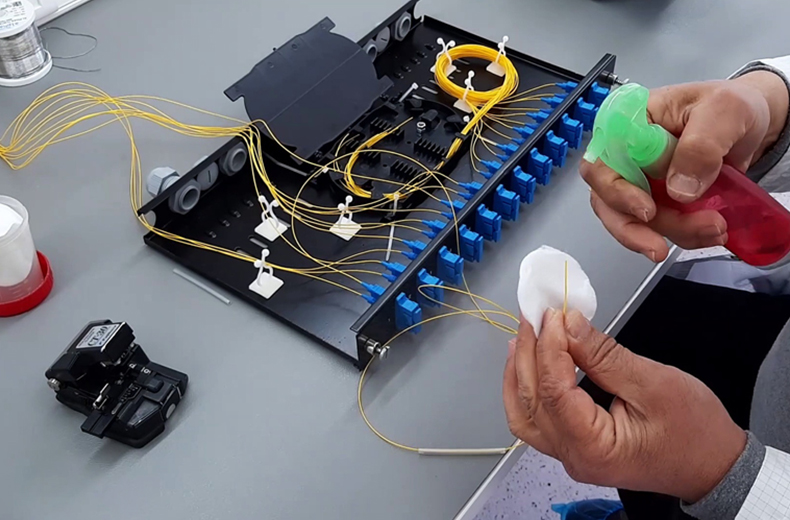
\includegraphics[width=10cm]{images/Fiber-Optik-Ek-ve-Sonlandirma}
    \caption{fibersonlandırma}
    \label{fig:fosonlandirma}
\end{figure}
\\
*F/O eki füzyon cihazı ile yapılır.2 tane cam tüpleri kaynatarak birbirine ekler.\\
İşlemler mikron seviyesinde yapıldığından kendi mikroskopu olan ve hassasiyeti yüksek olan cihazlar kullanılır. \\
F/O kablo testleri "OTDR" isimli cihaz  ile yapılır.
\section*{MAC ADRESİ VE ADRES ÇÖZÜMLEME}
Yerel ağlarda  haberleşmeyi sağlayan ethernet çerçevesinde(frame) 48 bitlik adres kullanılır.
MAC adresi 16'lık sayı sisteminde 12 tane karakter ile gösterilir.


\begin{table}[h]
    \centering
    \begin{tabular}{ll}
        16 bit & $\rightarrow$  $2^4$ 0000    \\
        48     & $\rightarrow$ 16 tane  $2^4$ \\
    \end{tabular}
\end{table}

İlk 6 karakterlik ilk 24 bit üretici kodunun son 6 karakter ise seri numarasını belirtir.Bir üretici aynı MAC adresiini birden fazla karar vermez.Dolyısıyla MAC adresleri dünyada tektir.
* Birden fazla aynı MAC adresi aynı ağ üzerinde(LAN,VLAN vb) olmamalıdır.

\begin{table}[h]
    \centering
    \begin{tabular}{ll}
        \textbf{Windows}                    & $\rightarrow$  CMD                           \\
        & $\rightarrow$  ipconfig                      \\
        & $\rightarrow$  getmac                        \\
        \textbf{ \textcolor{violet}{Linux}} & $\rightarrow$ \textcolor{violet}{ifconfig} \\
    \end{tabular}
\end{table}

\textbf{Adres Çözümleme} Ağdaki Bilgisayarlar başlangıçta diğer bilgisayarların mac adreslerini bilemez.
MAC adreslerini öğrenmek için;
\subsection*{ARP(Adress Resulotion Protocol) (Adres Cözümleme Protokolü)}
Bu protokol ikinci katmanda çalışır.Ağdaki Bilgisayarların MAC adreslerini öğrenmek ve bu cihazdaki ARP tablosunu güncellemek en temel görevdir.

SORU**
ARP tablosunda;statik kayıt ne işe yarar?
1970 de bilgisayar ağları tasarlanırken gelişimi hakkında kesin bilgi olmadığında statik(önü açık ) bırakılmıştır.
\subsection*{YAYIN ADRESİ(BROADCAST ADDRESS)}
Tüm yerel ağı temsil eden tek bir adrestir .Bu adrese gönderilen paket ağdaki tüm cihalara aynı anda uaştırılır.İkinci veya üçüncü katmanda yayın mesajı gelir.Yayın mesajlarında ne gibi fark vardır?
\begin{figure}[!ht]
    \includegraphics{images/Yayınadresitablosu}
    \caption{fibersonlandırma}
    \label{fig:fosonlandırma}
\end{figure}
\\
İkinci katmanda yayın adresi göndermek için çerçevedeki hedef mac adresindeki kısmında tüm bitler 1 yapılır.
Dolayısıyla hedef adresi FF:FF:FF:FF:FF:FF yapılır.Ağa yeni bağlanan her cihaz kendi mac ve IP adreslerini içeren bir yayın mesajı gönderir.
Her bilgisayarda ve anahtarda aynı ağdaki cihazlarla tutulan IP ve MAC adreslerinin tablosuna "ARP TABLOSU" denir. ARP Tablosu dinamik olarak güncellenir,ancak istenirse elle düzenleme ya da statik kayıt işlemi yapılabilir.
\subsubsection*{YAYIN ALANI}
Bilgisayarların doğrudan mac adresleriyle haberleştikleri alandır.Bir yayın paketi gönderildiğinde bunu alabilen tüm cihazlar aynı yayın alanındadır.
Bir bilgisayr kendi yayın alanında olmayan başka bir bilgisayarla haberleşmek için "ağ geçidinden" geçmek zorundadır.
\subsection*{ÇARPIŞMA ALANI}
Bir yayın alanı içerisinde bir veya birden fazla çarpışma alanı bulunur.Aynı çarpışma alanındaki bilgisayarlar birbirine gelen her paketi görürler,ancak sadece kendi mac adreslerine gelen her paketi görürler.
Çarpışma alanı aynı anda bir pc tarafından kullanılabilir.\\
İki PC aynı anda paket göndermek isterse çarpışma(collision) oluşur.Adını burdan alır.\\

\begin{figure}[ht]
    \centering
    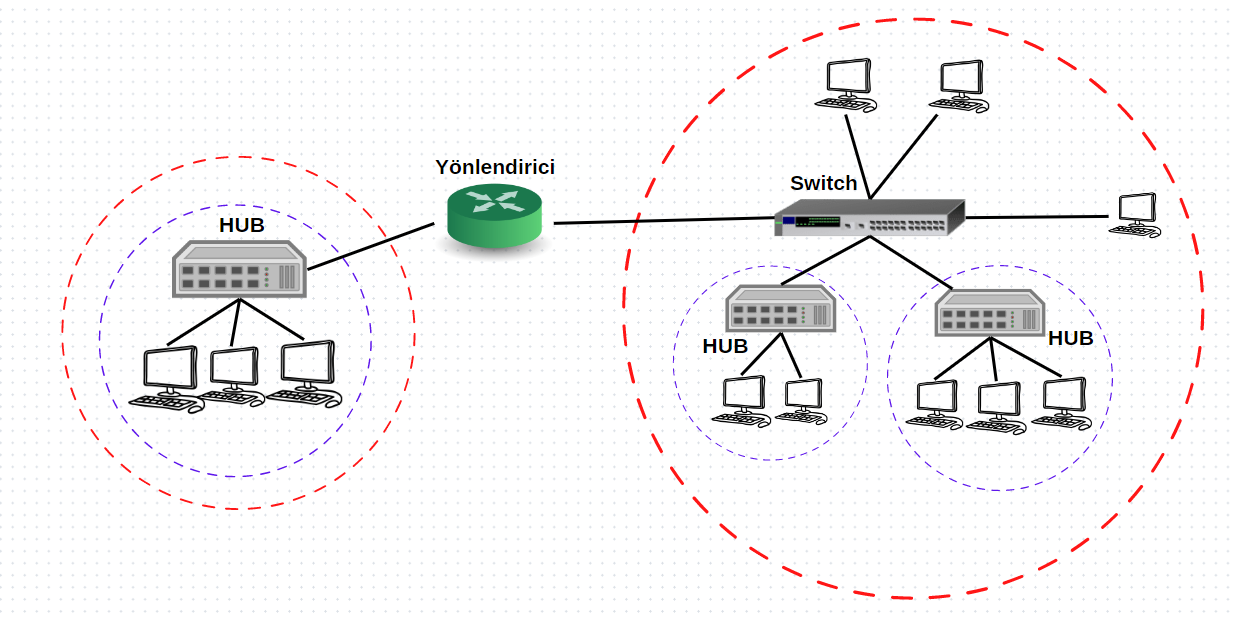
\includegraphics[width=8cm,height=6cm]{images/soru_1}
    \caption{Soru1}
    \label{fig:lan_vlan_ornegi1}
\end{figure}
 
1)Kaç tane yayın alanı vardır? 2 \\
2)Kaç tane çarpışma alanı vardır? 3\\
3)Her çarpışma alanında kaç tane bilgisayar vardır?\\
4)Her yayın alanında kaç tane bilgisayar vardır?\\
Birinci yayın alanında 3 tane\\
İkinci yayın alanında 8 tane \\

*YAYIN ALANI:mecburen ağ geçidi kullanılır.\\
*ÇARPIŞMA ALANI:Birbirlerinin verisini görecekler.


\begin{figure}[ht]
    \centering

    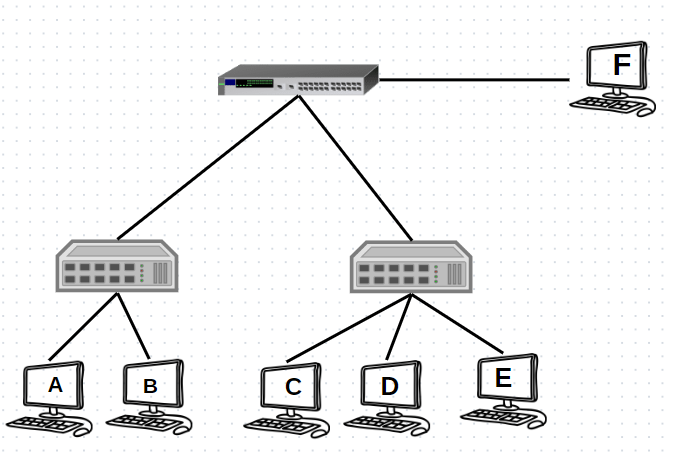
\includegraphics[width=8cm,height=6cm]{images/Soru2}
    \caption{Soru2}
    \label{fig:lan_vlan_ornegi}
\end{figure}
A ile B aynı anda paket gönderebilir mi? 
Yaçarpışma olur ya da sıra\\
B ile C aynı anda paket gönderebilir mi?\\
 B ile C aynı Pc gönderirse olur,ancak farklı olursa  aralarındaki topolojileri bilmediğimiz için bilemeyiz.\\
C yayın mesajı gönderdiğinde tüm pc'lere gider mi?\\
Evet tüm Pclere gider.\\
B ile C aynı arasındaki trafiği F görür mü?\\
Normal zamanda göremez.Ancak örneğin aynalama gibi işlemerde görebilir.\\
   

Anahtar üzerinde pc'lerin haricinde dış dünya ile iletişim kurmak için bağlantı yapılan porta "upink" poru denir.
Anahtarın bilgisayara bağlanan normal portlarına(bakır portlara 45 port) "giriş portu" denir.Genel olarak 100mb/s-1000mb/s  olurken "uplink portları" genellikle daha kapasiteli olur.
Anahtarları birbirinden ayıran bir diğer özellikte "demir gücü kapasitesi"anahtarın aynı  anda çevirebileceği trafik miktarına "switchfabric" ya da "through put"denir.
\subsubsection*{AĞ GEÇİTLERİ(GATEWAY)}
Önceden bahsedildği gibi anahtarlar çarpışma alanına geçemezler.Bu nedenle kablolara göre daha fazla tercih edilir.
Ancak anahtarlar da yayın trafiğini geçebilirer.Bünyesinde çok fazla anahtar bulunan yerel ağlar,yayın paketlerin çokluğu ağı hantallaştırır.Bu nedenle LAN'ları birbirinden çok alt ağa bölmek performansı arttıracaktır.
\textbf{Örnek Yayın Mesajları}\\
*IPV4 İIPV6 mesajları\\
*Komşuluk mesajları\\
*Donanım keşif mesajları\\
*Ip alma (DHCP)mesajları\\
*Virüs gibi kötü yazılımlar\\
\subsection*{Alt Ağa Bölmenin temel olarak iki yolu vardır}
\subsubsection*{Klasik Yöntem (Fiziksel Ağ Geçidi Kullanma)}
Klasik yöntemde herbir ağ için bir ağ geçidi kullanılması zorunludr.Dolayısıyla ciihazların,bağlantıları ve topolojilerin sınırları en önemli kısıtlardır.Bir vlan yapısında ise fiziksel bir müdahale olmadan hatta uzaktan bağlanarak ağ istenilen şekilde özelleştirilebilir.
\textbf{Sanal Ağlar(VLAN)}\\
yönlendirici,Kablosuz Ap,Güvenlik Duvarı,PC vb.

\begin{figure}[ht]
    \centering
    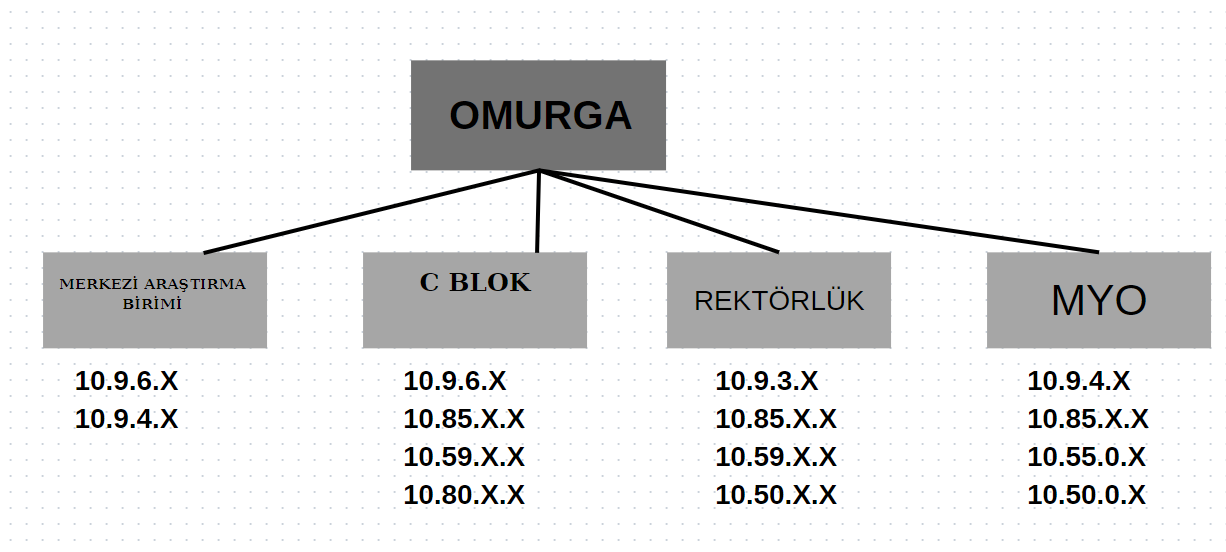
\includegraphics[width=8cm,height=6cm]{images/Soru3}
    \caption{VLAN}
    \label{fig:vlan_ornegi}
\end{figure}

Aynı ağ her yerde kullanılabiliyor.\\
Geleneksel yapıda ağları birbirinden ayrılması için ağ geçidi kullanılır\\
Bir anahtarda çok sayıda ağ(VLAN) kullanabiliyoruz.

\subsection*{SANAL AĞ(VLAN)KULLANMANIN AVANTAJLARI}
\begin{enumerate}[label=\alph*)]
    \item \textbf{Ağları Bölerek}: Her bir ağdaki pc sayısını azaltarak yayın alanını daraltmak ve performansı azaltmak
    \item \textbf{Esneklik}: Farklı coğrafyadaki bilgisayarlar aynı vlanda oabilir ya da aynı anahtar üzerinde birden fazla farklı vlan olabilir.
    \item \textbf{Güvenlik}: Birbirine erişimi kısıtlamaması gereken ağlar arasında erişim denetim listeleri(Access Control List(ACL)) oluşturularak erişim kısıtlanabilir.
    \item \textbf{İşletme Kolaylığı}: Ağlar küçük olduğunda sorunu çözmek kolaylaşır.Yani ağ eklemek ve mevcut ağları düzenlemek kolaylaşır.Ağ isimleri,IP grupları ve kullanım yerleri eşleştirilerek hiyerarşik sistemler oluşturulabilir.\\
    Ağ geçidi tanımı yönlendirme,prptokol çevirme veya güvenlik uygulaması gibi işlemleri yapan tüm cihazları kapsar.Sıradan bir PC ,3.katman(L3) anahtar,yönlendirici veya özel üretilmiş donanım olabilir.\\
    Ağ geçitleri üzerindeki ağ arayüzüne(interface) bağlı olarak ethernet,Frame Relay,ATM,PPPoE gibi protokollerin hepsinin kullanılabilme özelliğine sahip olduğundan bazı kaynaklardan protokol çevirici olarak adlandırılır.
\end{enumerate}
\begin{figure}[ht]
    \centering
    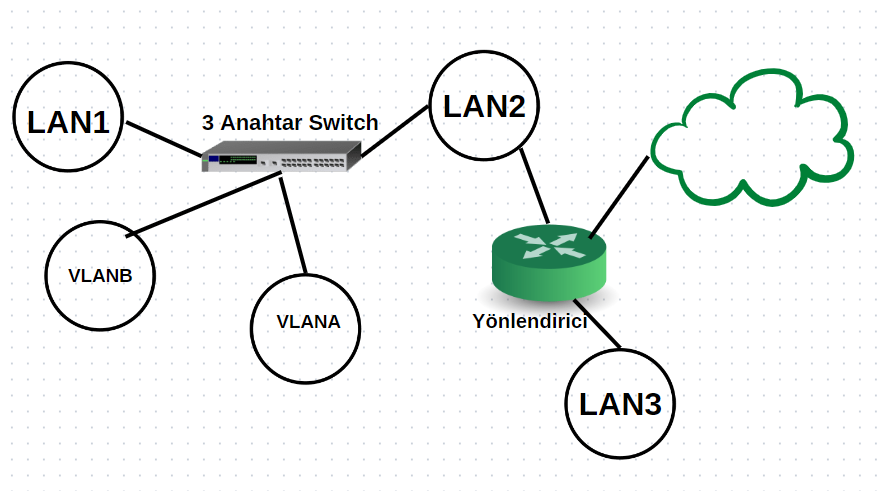
\includegraphics[width=8cm,height=6cm]{images/Vlanlar}
    \caption{LAN-VLAN}
    \label{fig:lan_vlan_sorusu}
\end{figure}


\section*{VLAN ANAHTARLAR}
Üzerinde sanal ağlar tanımlanabilen anahtarlardır.Sıradan anahtarlarda üstün olmasının en önemli sebebi ayarlanabilir olmasıdır.
Bu nedenle yönetilebilir anahtarlar da denmektedir.Vlan anahtarın üzerindeki portlar gruplandırılarak birden çok sanal ağ oluşturulabilir.Her bir sanal anahtar ayrı bir ağ gibi çalıştırılabilir.Bu sanal ağlara "VLAN" denir.Her bir vlan'ın kendine özel Vlan Id isminde bir tanımlayıcı numarası olur.
Anahtarları fizikse portları Vlan ID'leri ile eşleştirilerek ağlar düzenlenir.Aynı vlan numrasına sahip portlar aynı sanal ağa aittir.\\
Bazı durumlarda VLAN yapılandırılması portlardan ve fiziksel bağlantılardan bağımsız olarak yapılabilir.Örneğin pc'nin MAC adreslerine göre ya da kullanıcı kimlik doğrulama yöntemine göre (parola,parmak izi ) Vlan ataması yapılabilir.\\
Vlan anahtarlar kullanıldığında birden fazla sanal ağı oluşturursa bu alt ağlar arasında trafiğin yönlendirilmesi gerekmektedr.Bu yönlendirme işlemi anhtarın kendi üzerinde veya ayrı bir yönlendirici cihazla yapmak mümkündür.\\
Anahtar üzerinde yönlendirme yapılacaksa 3 katmanda(L3) çakıştırılacak bir anahtar kullanılmalıdır.\\
trunk: Anahtarın herhangi bir portundan birden fazla VLAN taşınması gerekiyorsa o port trunk olarak yapılandırılmalı.Bu bağlantıya da "trunk" denir.
\section*{ANAHTAR KULLANIM MİMARİSİ}
\begin{figure}[ht]
    \centering
    \includegraphics[width=8cm,height=6cm]{images/anahtarkullanımmimarisi}
    \caption{Anahtar-Kullanım-Mimarisi}
    \label{fig:anahtar_kullanım_mimarisi}
\end{figure}

1)OMURGA(CORE)\\
Üçüncü katman veya daha üstü anahtar kullanılır.Genellikle tüm Vlanlar burda oluşturulur.Ağın tüm yönlendirme yükü bunun üzerindedir.Bu nedenle genellikle yedekli kullanıır.Performansı çok fazladır.Binalar arası bağlantıyı sağlamak için kullanılır.Bu nedenle çok sayıda fiberoptik port sergilerler.Modüler yapıdadırlar,yani port sayıları ve türleri modüler halinde takılıp çıkartılabilir.Modülerin takıldığı yere "şase" denir.Fiziksel olarak çok yer kaplarlar ve pahalıdırlar.\\
2)Dağıtım(Distrubution)Katmanı \\
Omurga anahtarında bağlı olan ve binaların içerisinde küçük bir omurga gibi düşünebileceğimiz anahtarlardır.Omurga anahtarına göre daha ucuzdur.L2 veya L3 olabilir.\\
3)KENAR
Son kullanıcı cihazlarının bağlandığı anahtarlardır.Bu nedenle özel görevleri olabilir.\\
İhtiyaca göre :\\
802.1x(Kimlik Doğrulama)\\
PoE(802.3aaf) Enerji göndermek için kullanılır.\\
Captive Portal\\
Örnek:20 portlu bir VLAN anahtar 4  portlu bir ağ geçidine bağlanabiliyorAşağıdaki durumları yorumlayınız.\\
1)Her portun port sayısı 5'er tanedir.\\
Böyle bir zorunluluk yoktu\r.\\
2)Bir valan anahtar üzerine doğrudan bağlanacak PC sayısı 16'dır\\
16 tane de olabilir daha fazla da olabilir.\\
3)Her vlana atanmış portlar ardışık olmak zorundadır\\
Öyle bir şey yok.Esneklik özelliği vardır . 
